% This LaTeX file contains your written lab questions.  You may answer these
% questions just by inserting your answer into this document.
%
% If you're unfamiliar with LaTeX, see the document LearningLaTeX.tex in this
% same directory.  It contains a brief explanation and a few snippets of LaTeX
% code to get you started; in fact, it should have everything you need to
% complete this assignment.
%
% Also see the example file in examples/week-04/bigO.tex
\documentclass{article}

\usepackage{amsmath}
\usepackage{amssymb}
\usepackage{amsthm}
\usepackage{graphicx}
\usepackage{tabu}
\usepackage{float}

\begin{document}

    \section{MergeSort}

    See the source code file \texttt{mergeSort.cpp} and the tests given in
    \texttt{tests.cpp}.

    \section{Big-O Proofs}
	
    \vspace{2mm}
    \noindent {\large\textbf{Problem 1.}} Show that $6n^2−n+4$ is $O(n^2)$.

    \begin{proof}
    	Let $f(n) = 6n^2 - n + 4$. We want to find constants $c$ and $n_0$ such that for all $n>n_0$, 
    	\begin{equation*}
    	f(n) < c \cdot n^2.
    	\end{equation*}
    	Let $c = 7$ and $n_0 = 10$. Consider the function $f(n) - c \cdot n^2 =6n^2 - n + 4 - 7n^2 =  -n^2 - n + 4.$ For all $n>n_0$, $f(n) - c \cdot n^2 = -n^2 - n + 4<0$. Therefore for the given values of $n_0$ and $c$, $f(n) - c \cdot n^2 < 0$ for all $n> n_0$, which is equivalent to saying:
    	\begin{equation}
    	f(n) < c \cdot n^2,
    	\end{equation}
    	for all $n>n_0$ as desired. 
    \end{proof}

    \vspace{1cm}
    \noindent {\large\textbf{Problem 2.}} Show that $n^3 + 8n^2 - 12$ is $O(n^3)$.
	\begin{proof}
		Let $c=10$ and $n_0=10$. $f(n) = n^3 + 8n^2 -12$ and $c \cdot n^3 = 10n^3$. For all $n>n_0$, $f(n) - cn^3 = -9n^3 + 8n^2 -12 < 0$. Therefore:
		\begin{equation}
		f(n) < c \cdot n^3,
		\end{equation}
		for all $n>n_0$ as desired.
	\end{proof}

    \vspace{1cm}
    \newpage
    \section{Mystery Functions}

    %%%%%%%%%%%%%%
    %%%% TODO %%%%
    %%%%%%%%%%%%%%
    % Give your explanation of each of the mystery functions here.
    
    General approach: For high values of $n$, the power of an upper bound function is the dominant factor in the difference in runtime with respect to other functions. First, we are going to list
    the least upper bound functions for each of the lettered functions.
    
    \subsection{Obtaining the upper bounds.}
    \begin{enumerate}
    	\item[A] The for loop is iterated $n$ times, with one operation per iteration. Therefore $\hat O(fnA(n)) = n$.
    	\item[B] The for loop is iterated $4n$ times, with one operation per iteration. Therefore $\hat O(fnB(n)) = 4n$.
    	\item[C] The inner `j' for loop is iterated $n$ times; the outer `i' for 
    	loop is iterated $n$ times as well. Therefore $\hat O(fnC(n)) = n^2$. 
    	\item[D] The for loop is iterated $n^3$ times, with two operations per iteration. Therefore $\hat O(fnD(n)) = 2n^3$.
    	\item[E] The inner `j' for loop is iterated $n^2$ times; the outer `i' for loop is iterated $n^2$ times as well. Therefore $\hat O(fnE(n)) = n^2 \cdot n^2 = n^4$. 
    	\item[F] The inner `j' while loop is iterated $10$ times, with two operations per iteration; the outer `i' for loop is iterated $n^2$ times. Therefore $\hat O(fnF(n)) = \cdot 2 \cdot 10 \cdot n^2 = 20 n^2$.
    \end{enumerate} 
    
    
    \begin{figure}[H]
    	\centering
	    \begin{tabular}{c|c}
	    	function letter & upper bound \\
	    	\hline
	    	A & $n$ \\
	    	B & $4n$ \\
	    	C & $n^2$ \\
	    	D & $n^3$ \\
	    	E & $n^4$ \\
	    	F & $20*n^2$
	    \end{tabular}
    	\caption{For convenience, the table of upper bounds for the lettered functions. }
    \end{figure}
	
	\subsection{Comparisons and conclusions.}
	Referring to figure 2 below, we can see that with all functions plotted, $f3$ has the longest runtime against other functions especially at large values of $n$. Therefore the upper bound of $f3$ has the highest power. According to figure 1, mystery function $f3$ is $fE$ which has the highest power. 
	\begin{figure}[H]
	    \begin{center}
	       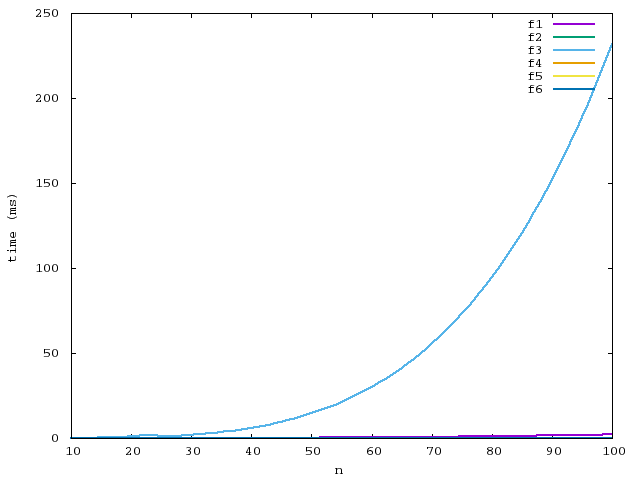
\includegraphics[width=0.5\textwidth]{Evidence_1.png}
	    \end{center}
    	\caption{Runtime vs $n$ with $n\in [10,100]$.}
	\end{figure}
	
	Referring to figure 3 below, excluding mystery function $f3$, $f1$ has the longest runtime against the remaining functions especially at large values of $n$. Therefore the upper bound of $f1$ has the highest power among the remaining mystery functions. According to figure 1, mystery function $f1$ is $fD$ which has the highest power. 
	\begin{figure}[H]
		\begin{center}
			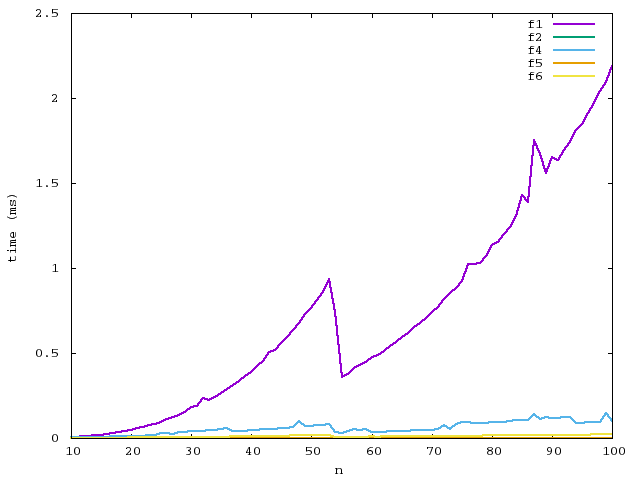
\includegraphics[width=0.5\textwidth]{Evidence_2.png}
		\end{center}
		\caption{Runtime vs $n$ with $n\in [10,100]$.}
	\end{figure}
	
	Referring to figure 4 below, excluding mystery functions $f3$ and $f1$, $f4$ and $f6$ have significantly longer runtime against the remaining functions especially at large values of $n$. Therefore the upper bound of $f4$ and $f6$ have the highest power among the remaining mystery functions. Furthermore, it is very likely that the uppder bounds of $f4$ and $f6$ are off by only a constant of proportionality. Therefore we can conclude that according to figure 1, $f4$ which has a larger constant of proportionality is $fF$ and $f6$ is $fC$.
	\begin{figure}[H]
		\begin{center}
			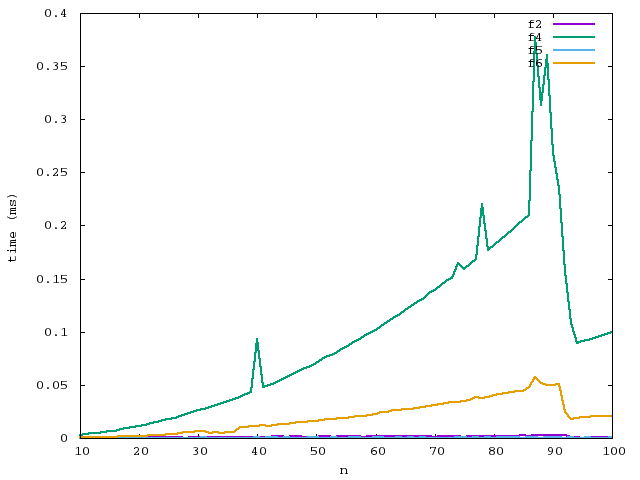
\includegraphics[width=0.5\textwidth]{Evidence_3.png}
		\end{center}
		\caption{Runtime vs $n$ with $n\in [10,100]$.}
	\end{figure}
	
	Referring to figure 1, the upper bounds of $f2$ and $f5$, by process of elimination should have the lowest power. According to figure 5, the functional behavior of runtime vs $n$ is similar between $f2$ and $f5$. Thus $f2$ should be $fB$ which has a higher constant of proportionality. And similarly $f5$ should be $fA$.
	\begin{figure}[H]
		\begin{center}
			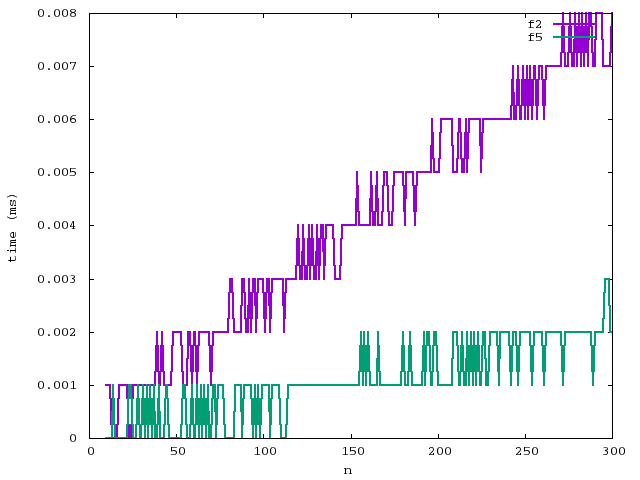
\includegraphics[width=0.5\textwidth]{Evidence_4.png}
		\end{center}
		\caption{Runtime vs $n$ with $n\in [10,100]$.}
	\end{figure}

	Below is a compiled table of results:
	
	\begin{figure}[H]
		\centering
		\begin{tabular}{c|c}
			mystery function & corresponding lettered function \\
			\hline
			$f1$ & $fD$ \\
			$f2$ & $fB$ \\
			$f3$ & $fE$ \\
			$f4$ & $fF$ \\
			$f5$ & $fA$ \\
			$f6$ & $fC$
		\end{tabular}
		\caption{Table of results.}
	\end{figure}
	
    % To include a png file, use the \includegraphics command
    % e.g. if you have a file 56.png comparing functions 5 and 6,
    % include it with the following command
    % \begin{center}
    %   \includegraphics[width=0.8\textwidth]{56.png}
    % \end{center}
    
    
\end{document}
